% ==================================================================
% Figure insertion snippets — CASPer major revision
% ==================================================================

% --- Main Figure 2: Random vs Cluster Split Performance ---
\begin{figure}[t]
\centering
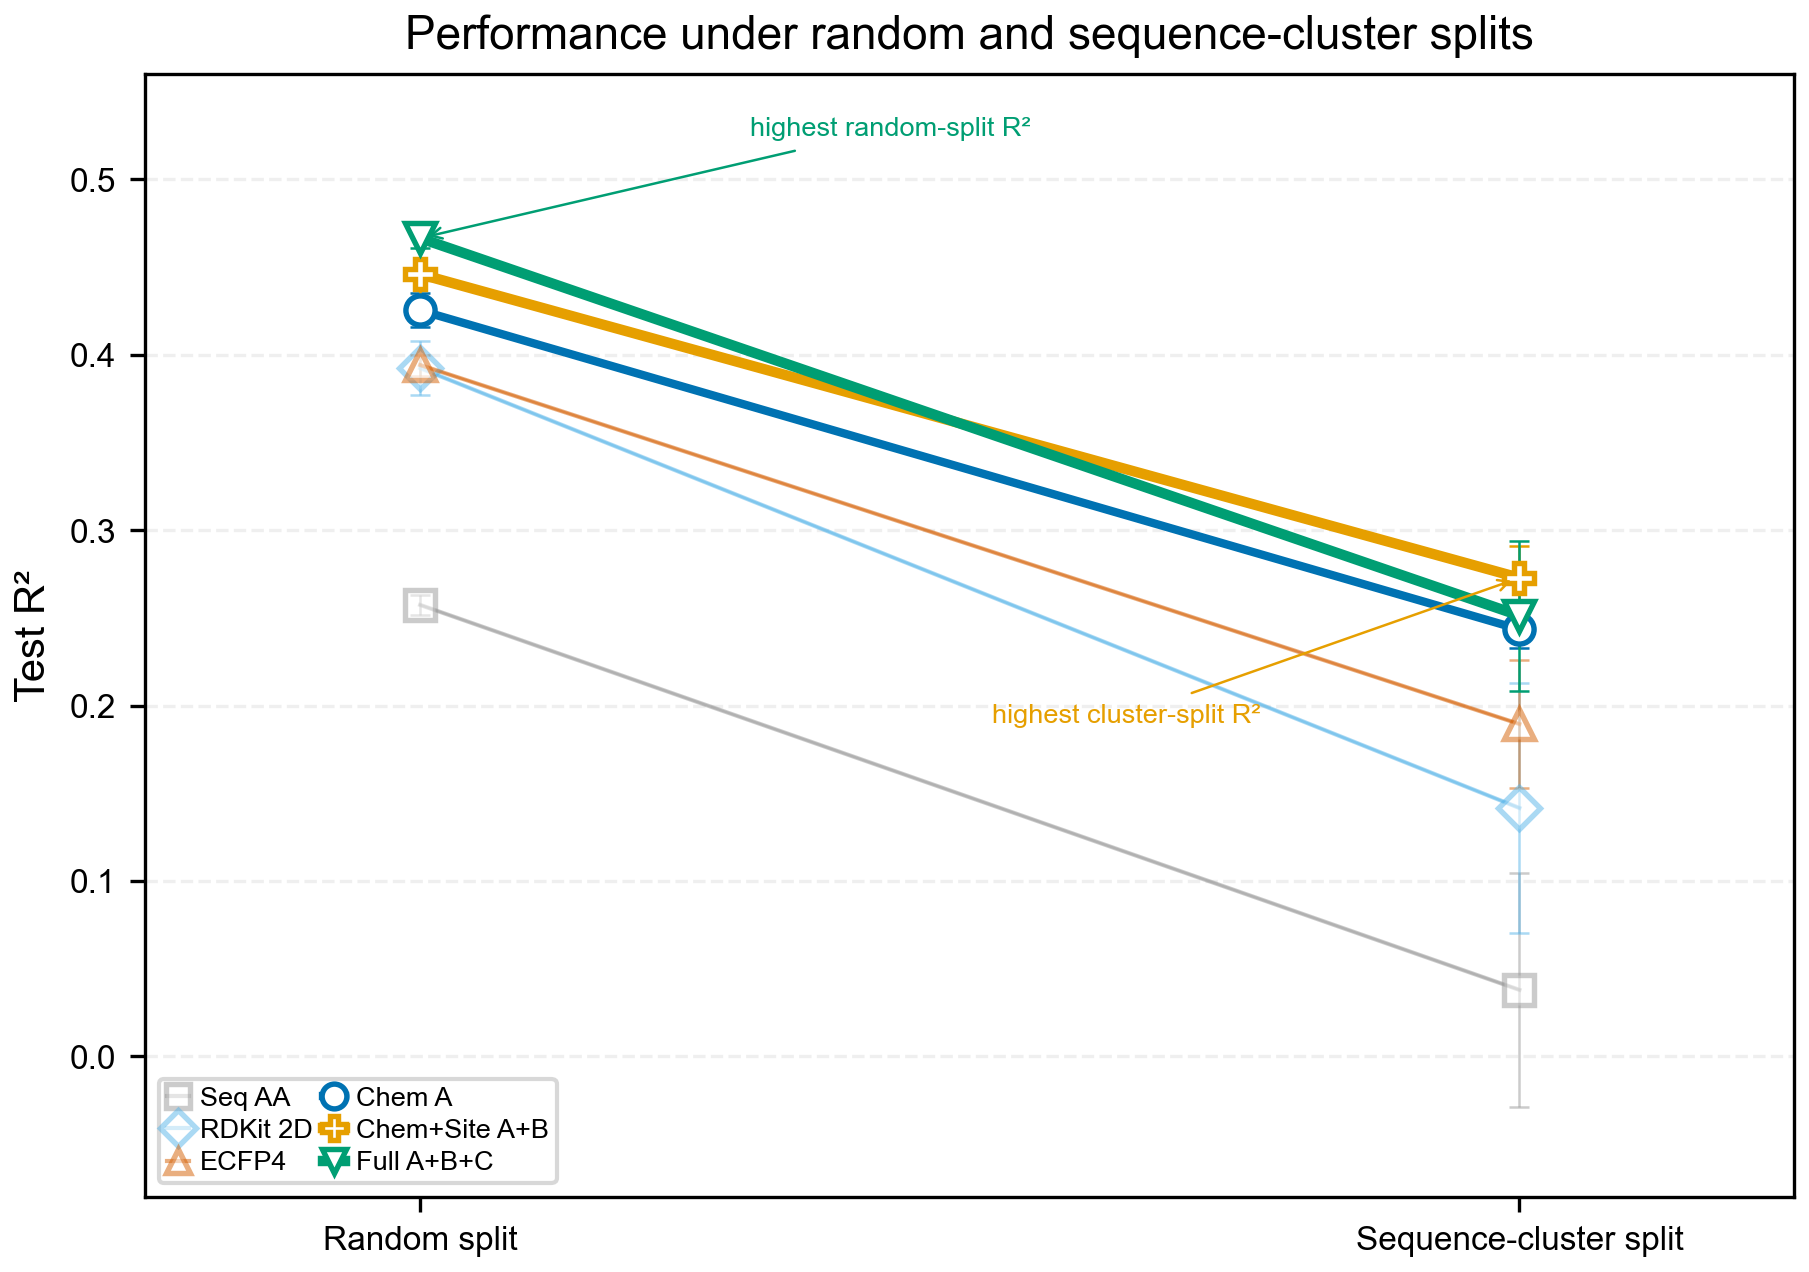
\includegraphics[width=0.92\textwidth]{figures/revision/fig2_random_cluster_slope.pdf}
\caption{%
Performance under random and sequence-cluster splits.
Each line connects a model's test R$^2$ from the random split to the
sequence-cluster split.  Full A+B+C achieves the highest random-split
R$^2$, while Chem+Site~A+B is the most robust model under the more
challenging cluster split.  All models lose performance in the cluster
regime, consistent with the increased difficulty of scaffold-shift
generalisation.}
\label{fig:random_cluster_slope}
\end{figure}

% --- Main Figure 3: Descriptor-set Comparison ---
\begin{figure}[t]
\centering
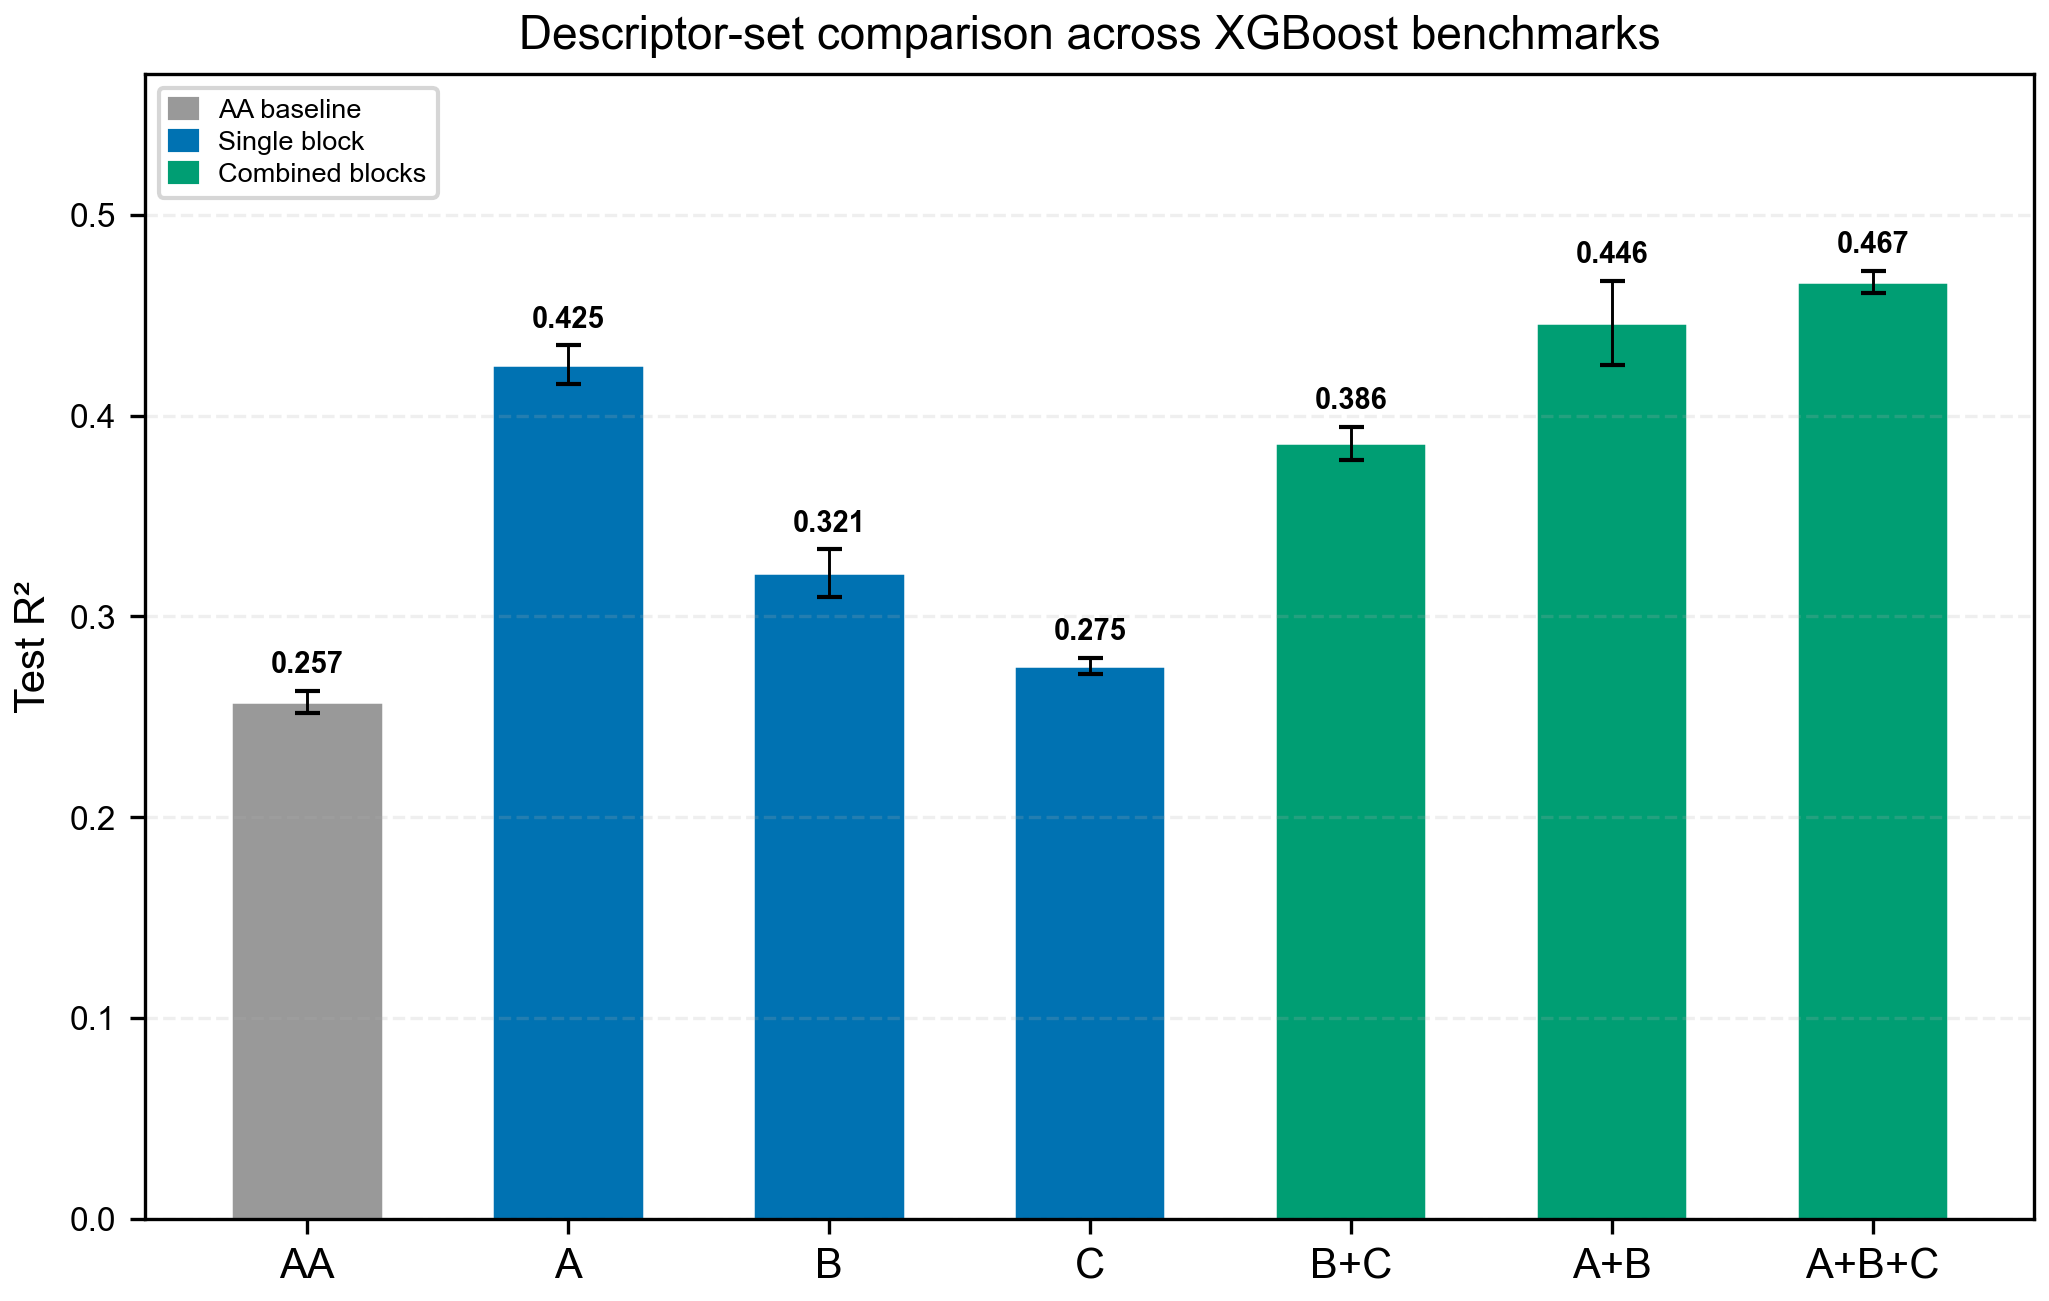
\includegraphics[width=0.88\textwidth]{figures/revision/fig3_descriptor_ablation.pdf}
\caption{%
Descriptor-set comparison across XGBoost benchmarks.
Bars show test R$^2$ for each descriptor set (A = edit chemistry;
B = explicit site; C = scaffold/multi-edit context).
Values for AA, A, A+B, and A+B+C are from the main benchmark
(5-seed, Optuna~50); values for B, C, and B+C are from the
estimator-comparison XGBoost row (5-seed, Optuna~10).
The additive formulation $f(S,E,A) \approx g_{\mathrm{A}}(E) +
h_{\mathrm{B}}(S,A) + c_{\mathrm{C}}(S,E,A)$ is shown for reference.}
\label{fig:descriptor_ablation}
\end{figure}

% --- Main Figure 4: SHAP Group Attribution ---
\begin{figure}[t]
\centering
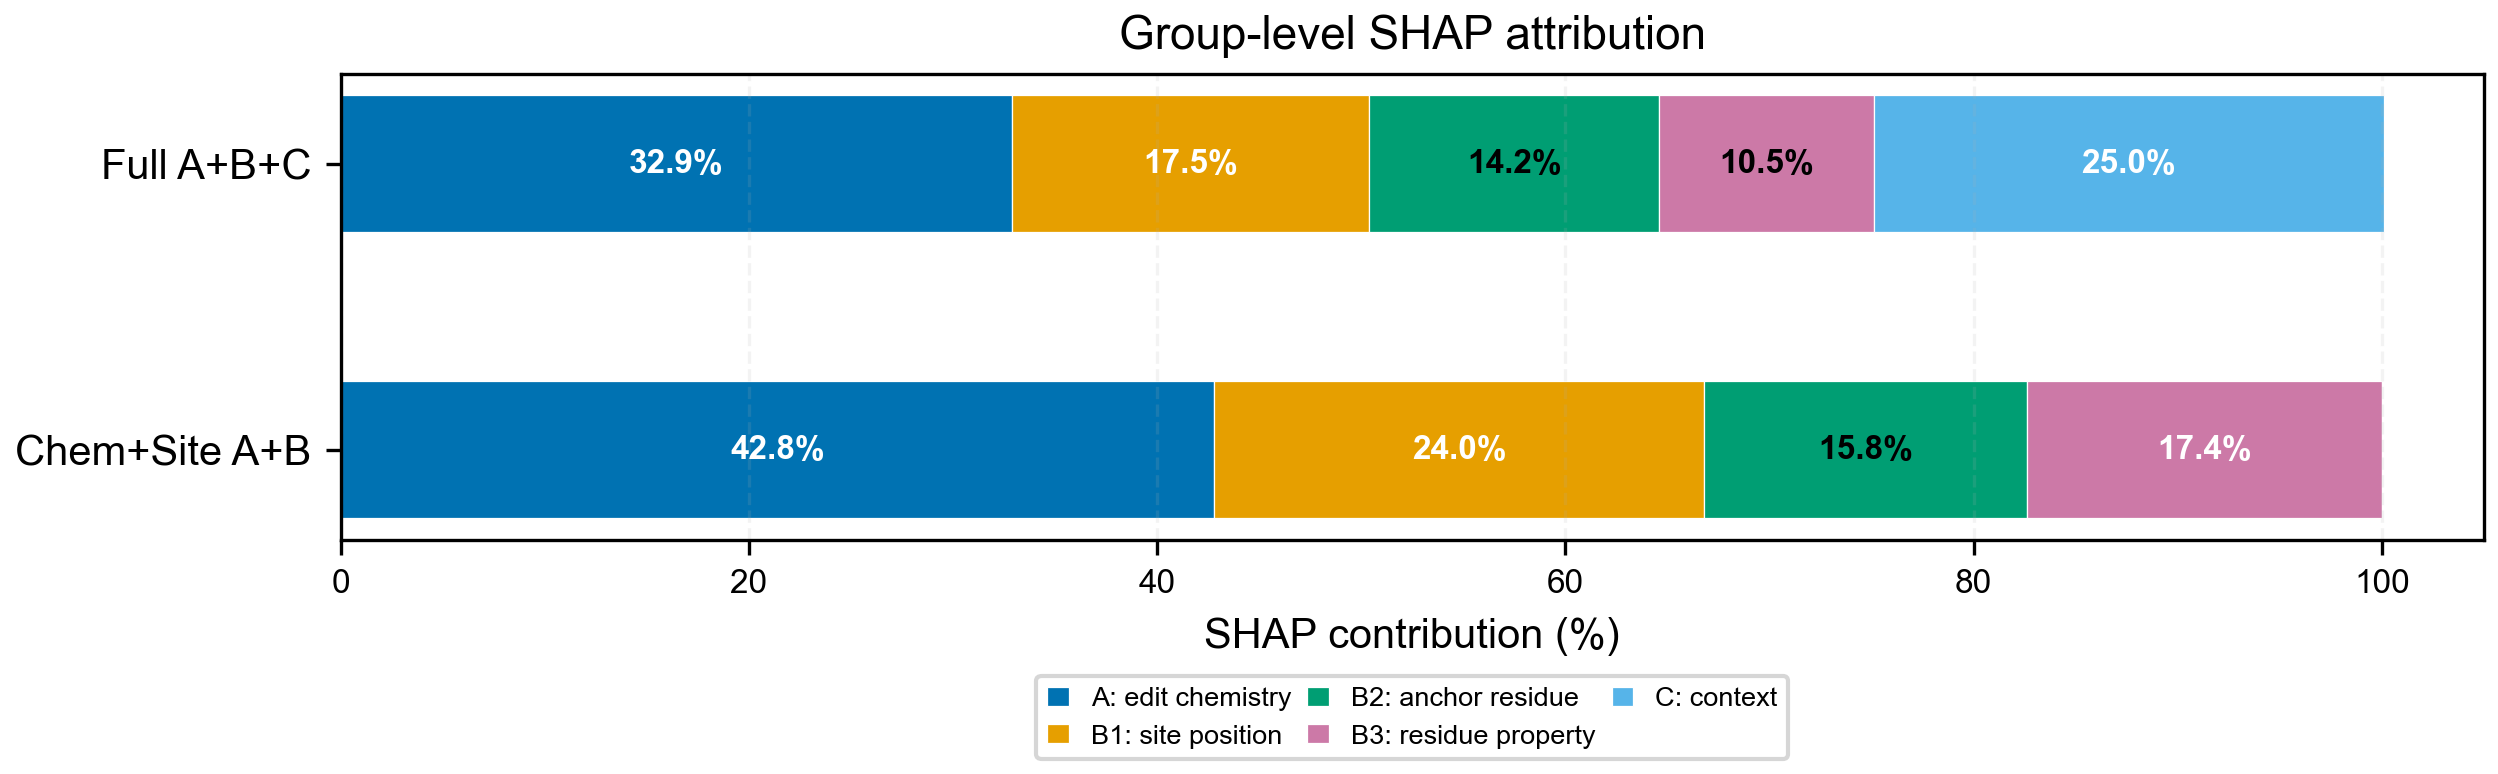
\includegraphics[width=0.75\textwidth]{figures/revision/fig4_shap_group_attribution.pdf}
\caption{%
Group-level SHAP attribution for Full~A+B+C and Chem+Site~A+B
XGBoost models.  SHAP values were aggregated by descriptor block:
edit chemistry (A), site position (B1), anchor residue (B2),
residue property (B3), and context (C).  Edit chemistry is the
dominant contributor but far from exclusive: site and context
descriptors together account for approximately two-thirds of the
total attribution in the full model, confirming a chemistry-first
but not chemistry-only representation.  The Chem+Site~A+B model
has no C-context features by construction.}
\label{fig:shap_group_attribution}
\end{figure}

% --- Main Figure 5: Estimator Heatmap ---
\begin{figure}[t]
\centering
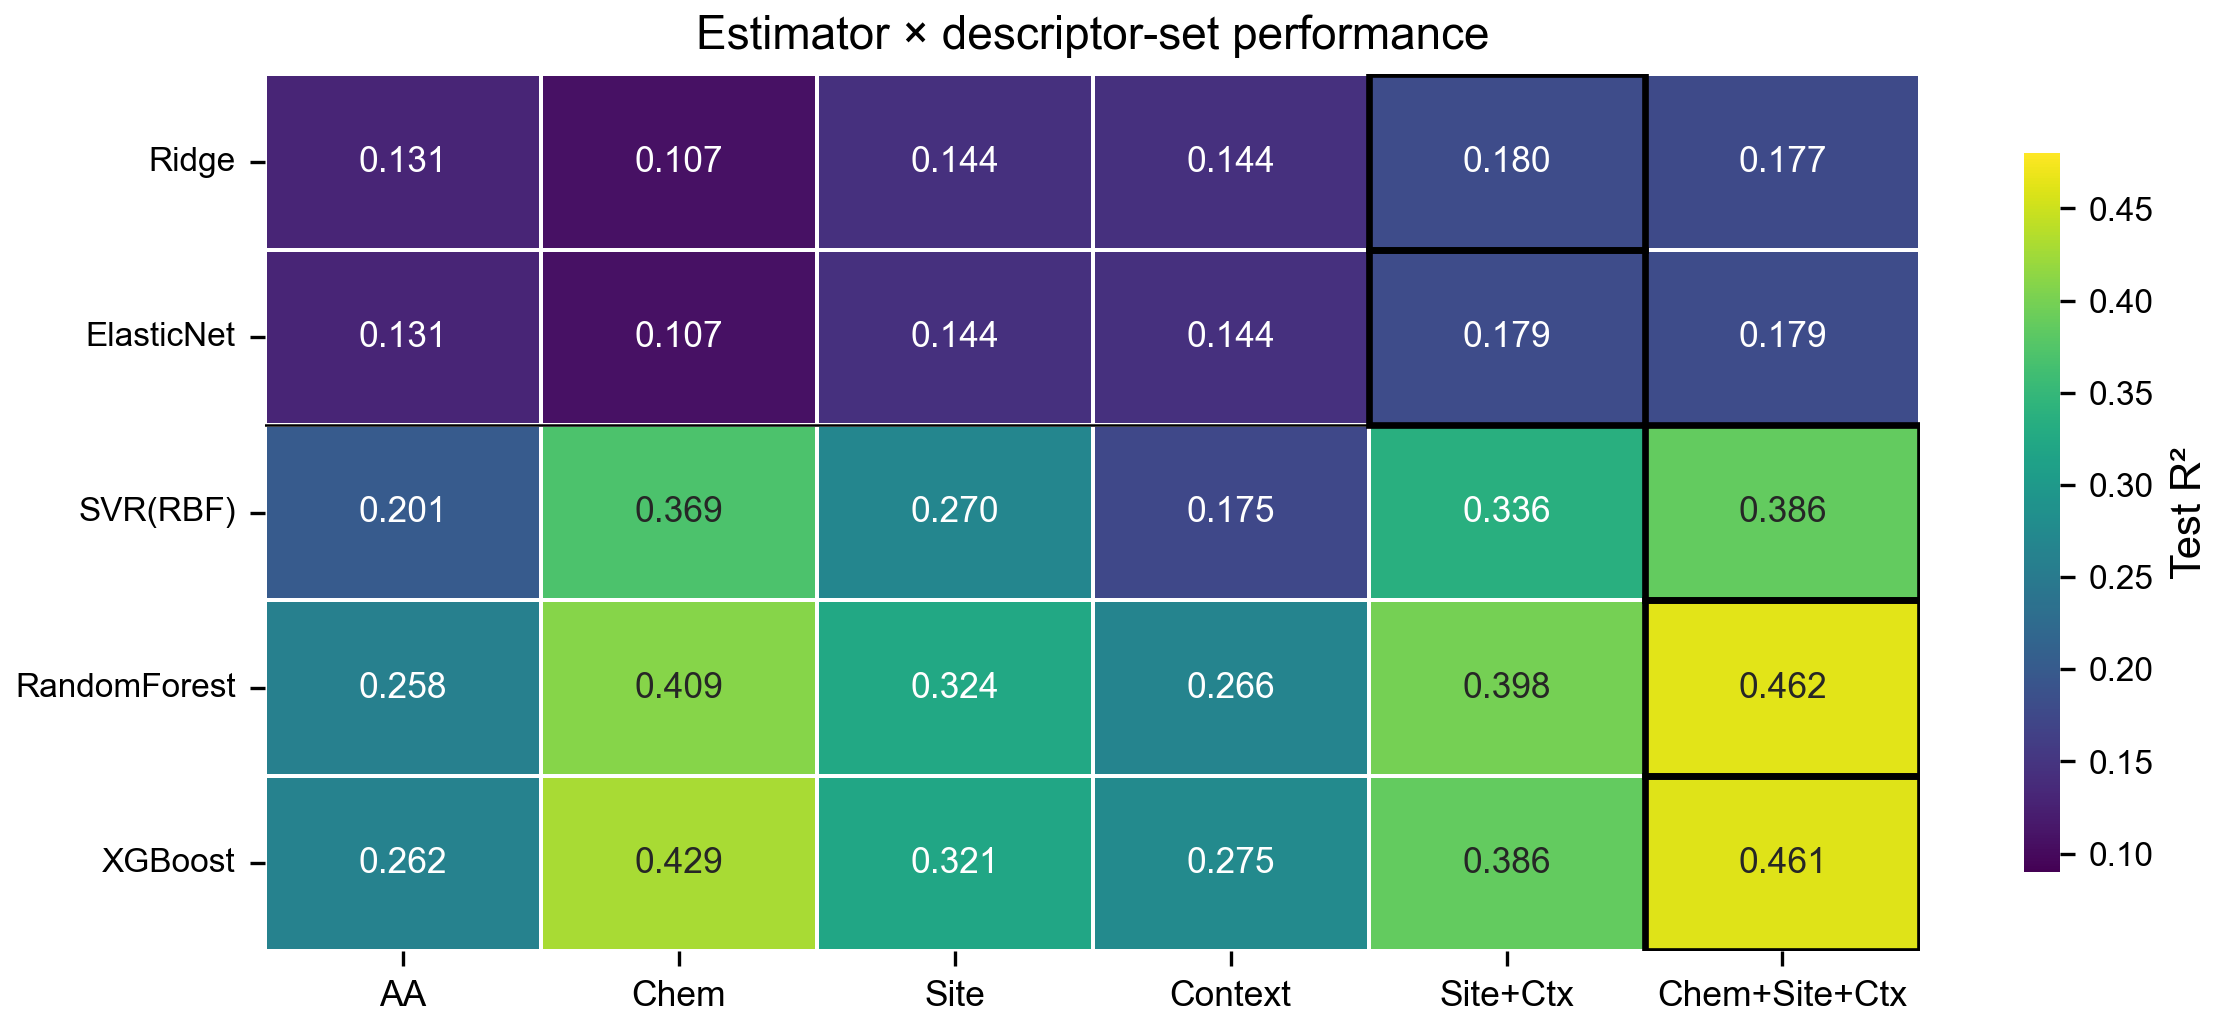
\includegraphics[width=0.92\textwidth]{figures/revision/fig5_estimator_heatmap.pdf}
\caption{%
Estimator $\times$ descriptor-set performance (test R$^2$).
Linear estimators (Ridge, ElasticNet) are unable to exploit the
chemistry--site--context combination; non-linear tree and kernel
methods (RandomForest, SVR(RBF), XGBoost) show monotonic gains
from chemistry to the full descriptor set.  The best value in each
row is highlighted with a bold border.}
\label{fig:estimator_heatmap}
\end{figure}

% --- Main Figure 6: Temporal \& Scaffold-Focused Ranking ---
\begin{figure}[t]
\centering
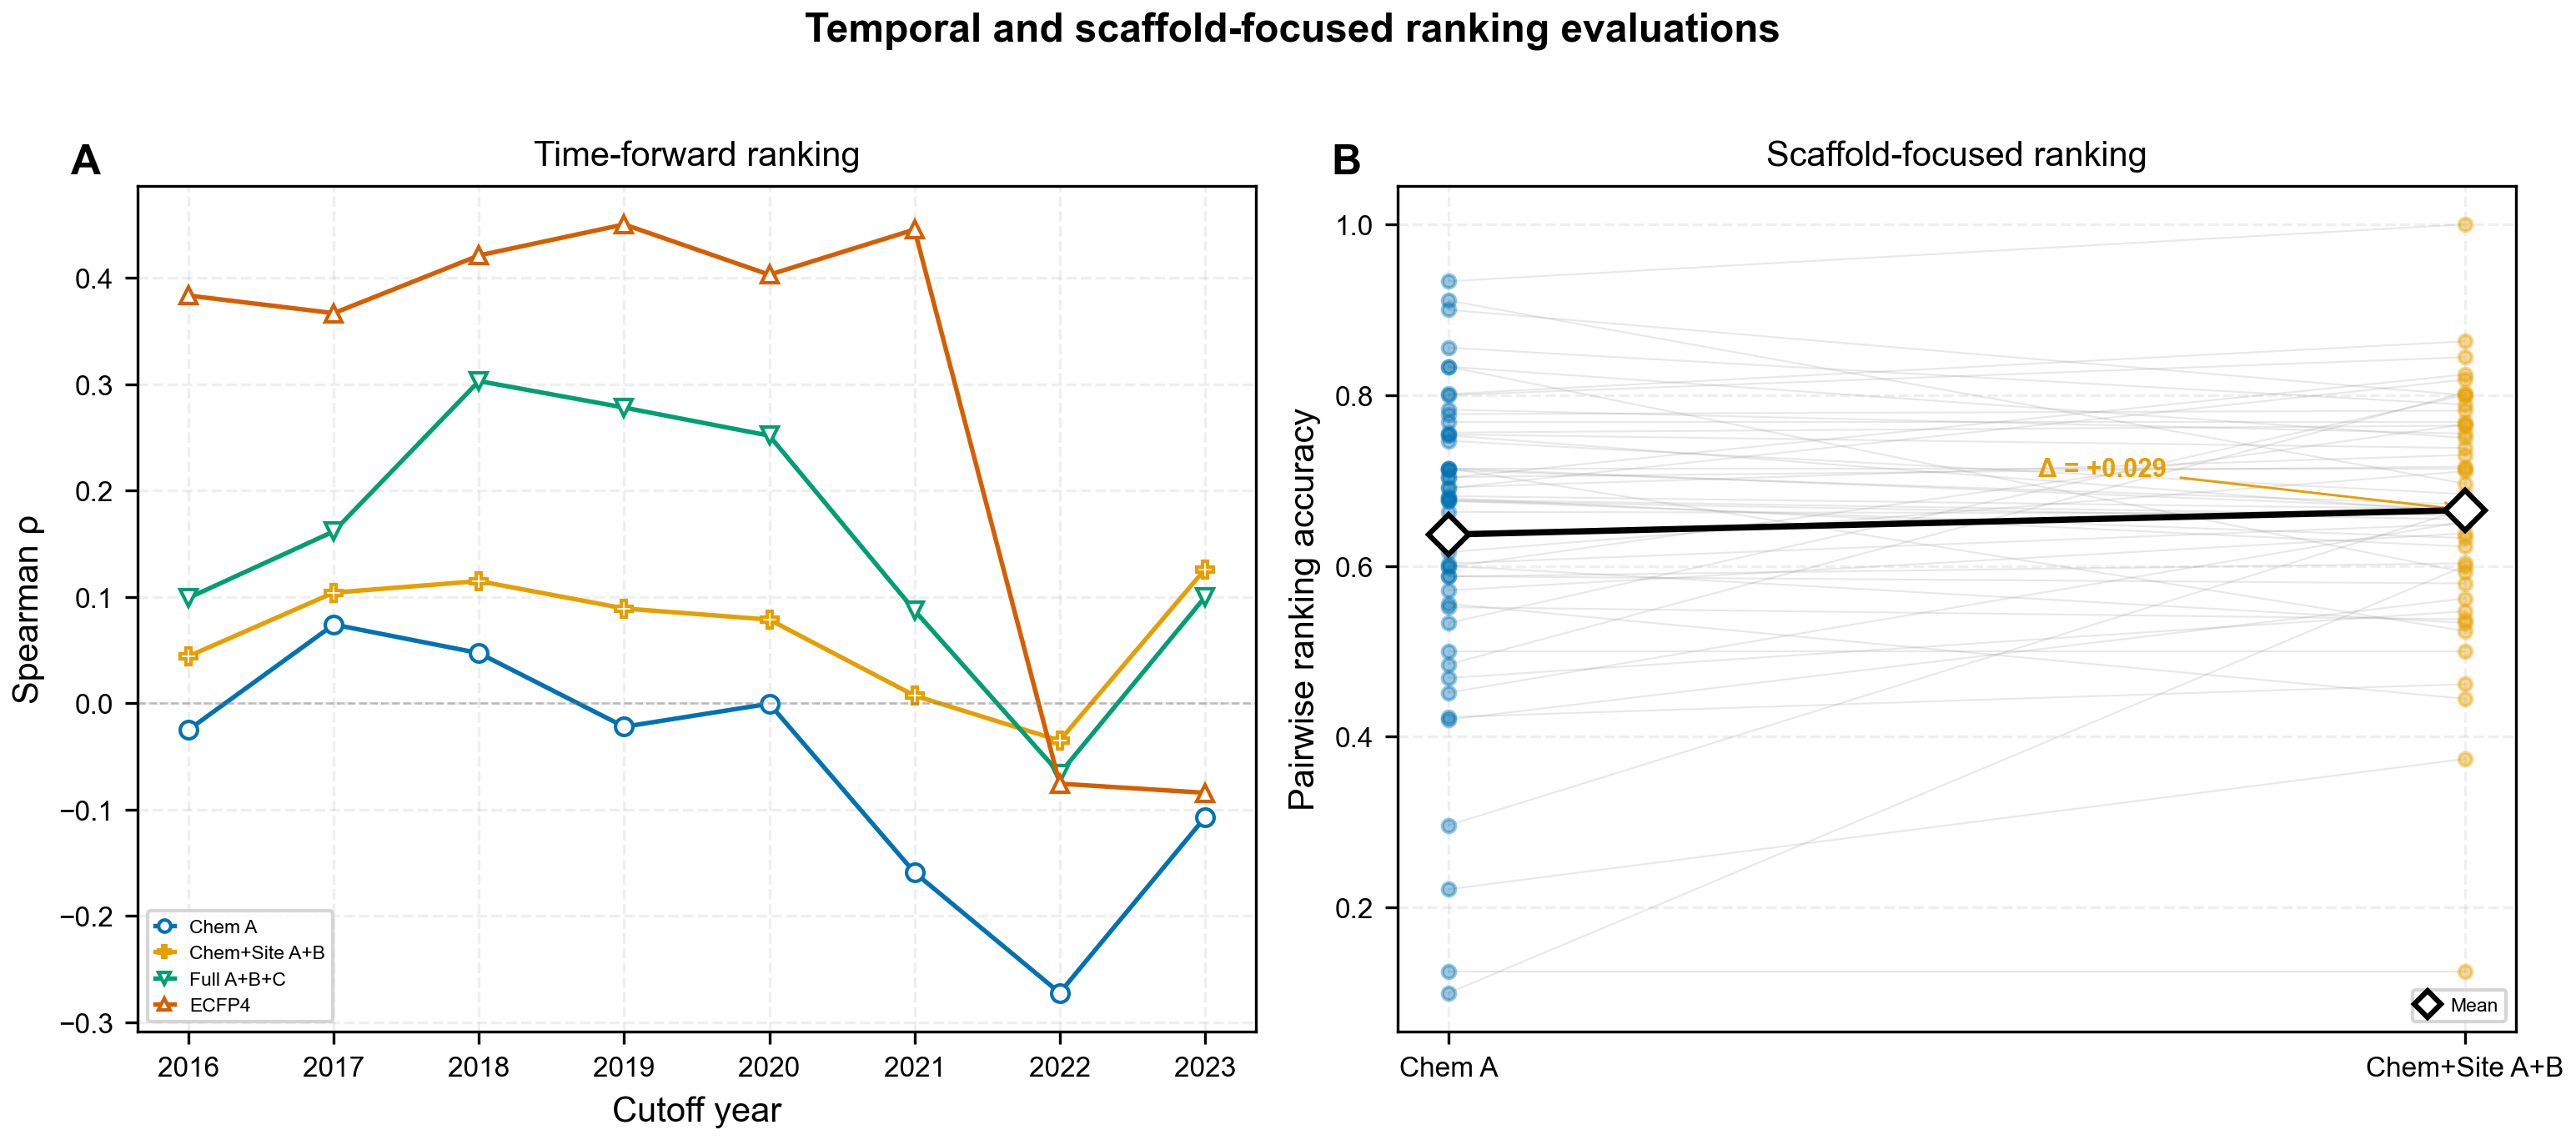
\includegraphics[width=\textwidth]{figures/revision/fig6_temporal_scaffold_ranking.pdf}
\caption{%
Temporal and scaffold-focused ranking evaluations.
(\textbf{A}) Time-forward ranking: Spearman $\rho$ across
publication-year cutoffs.  ECFP4 fingerprints provide the most stable
ranking under temporal shift, whereas descriptor-based models show
weaker generalisation, consistent with the harder regime of
extrapolating to future chemical space.
(\textbf{B}) Scaffold-focused ranking: paired per-family pairwise
accuracy for Chem~A and Chem+Site~A+B across 49 peptide scaffold
families.  Chem+Site~A+B achieves a higher mean accuracy (black
diamonds), demonstrating practical value for prioritising analogues
within a given scaffold.}
\label{fig:temporal_scaffold_ranking}
\end{figure}

% --- Supplementary Figure S1: Parser Audit Flow ---
\begin{figure}[t]
\centering
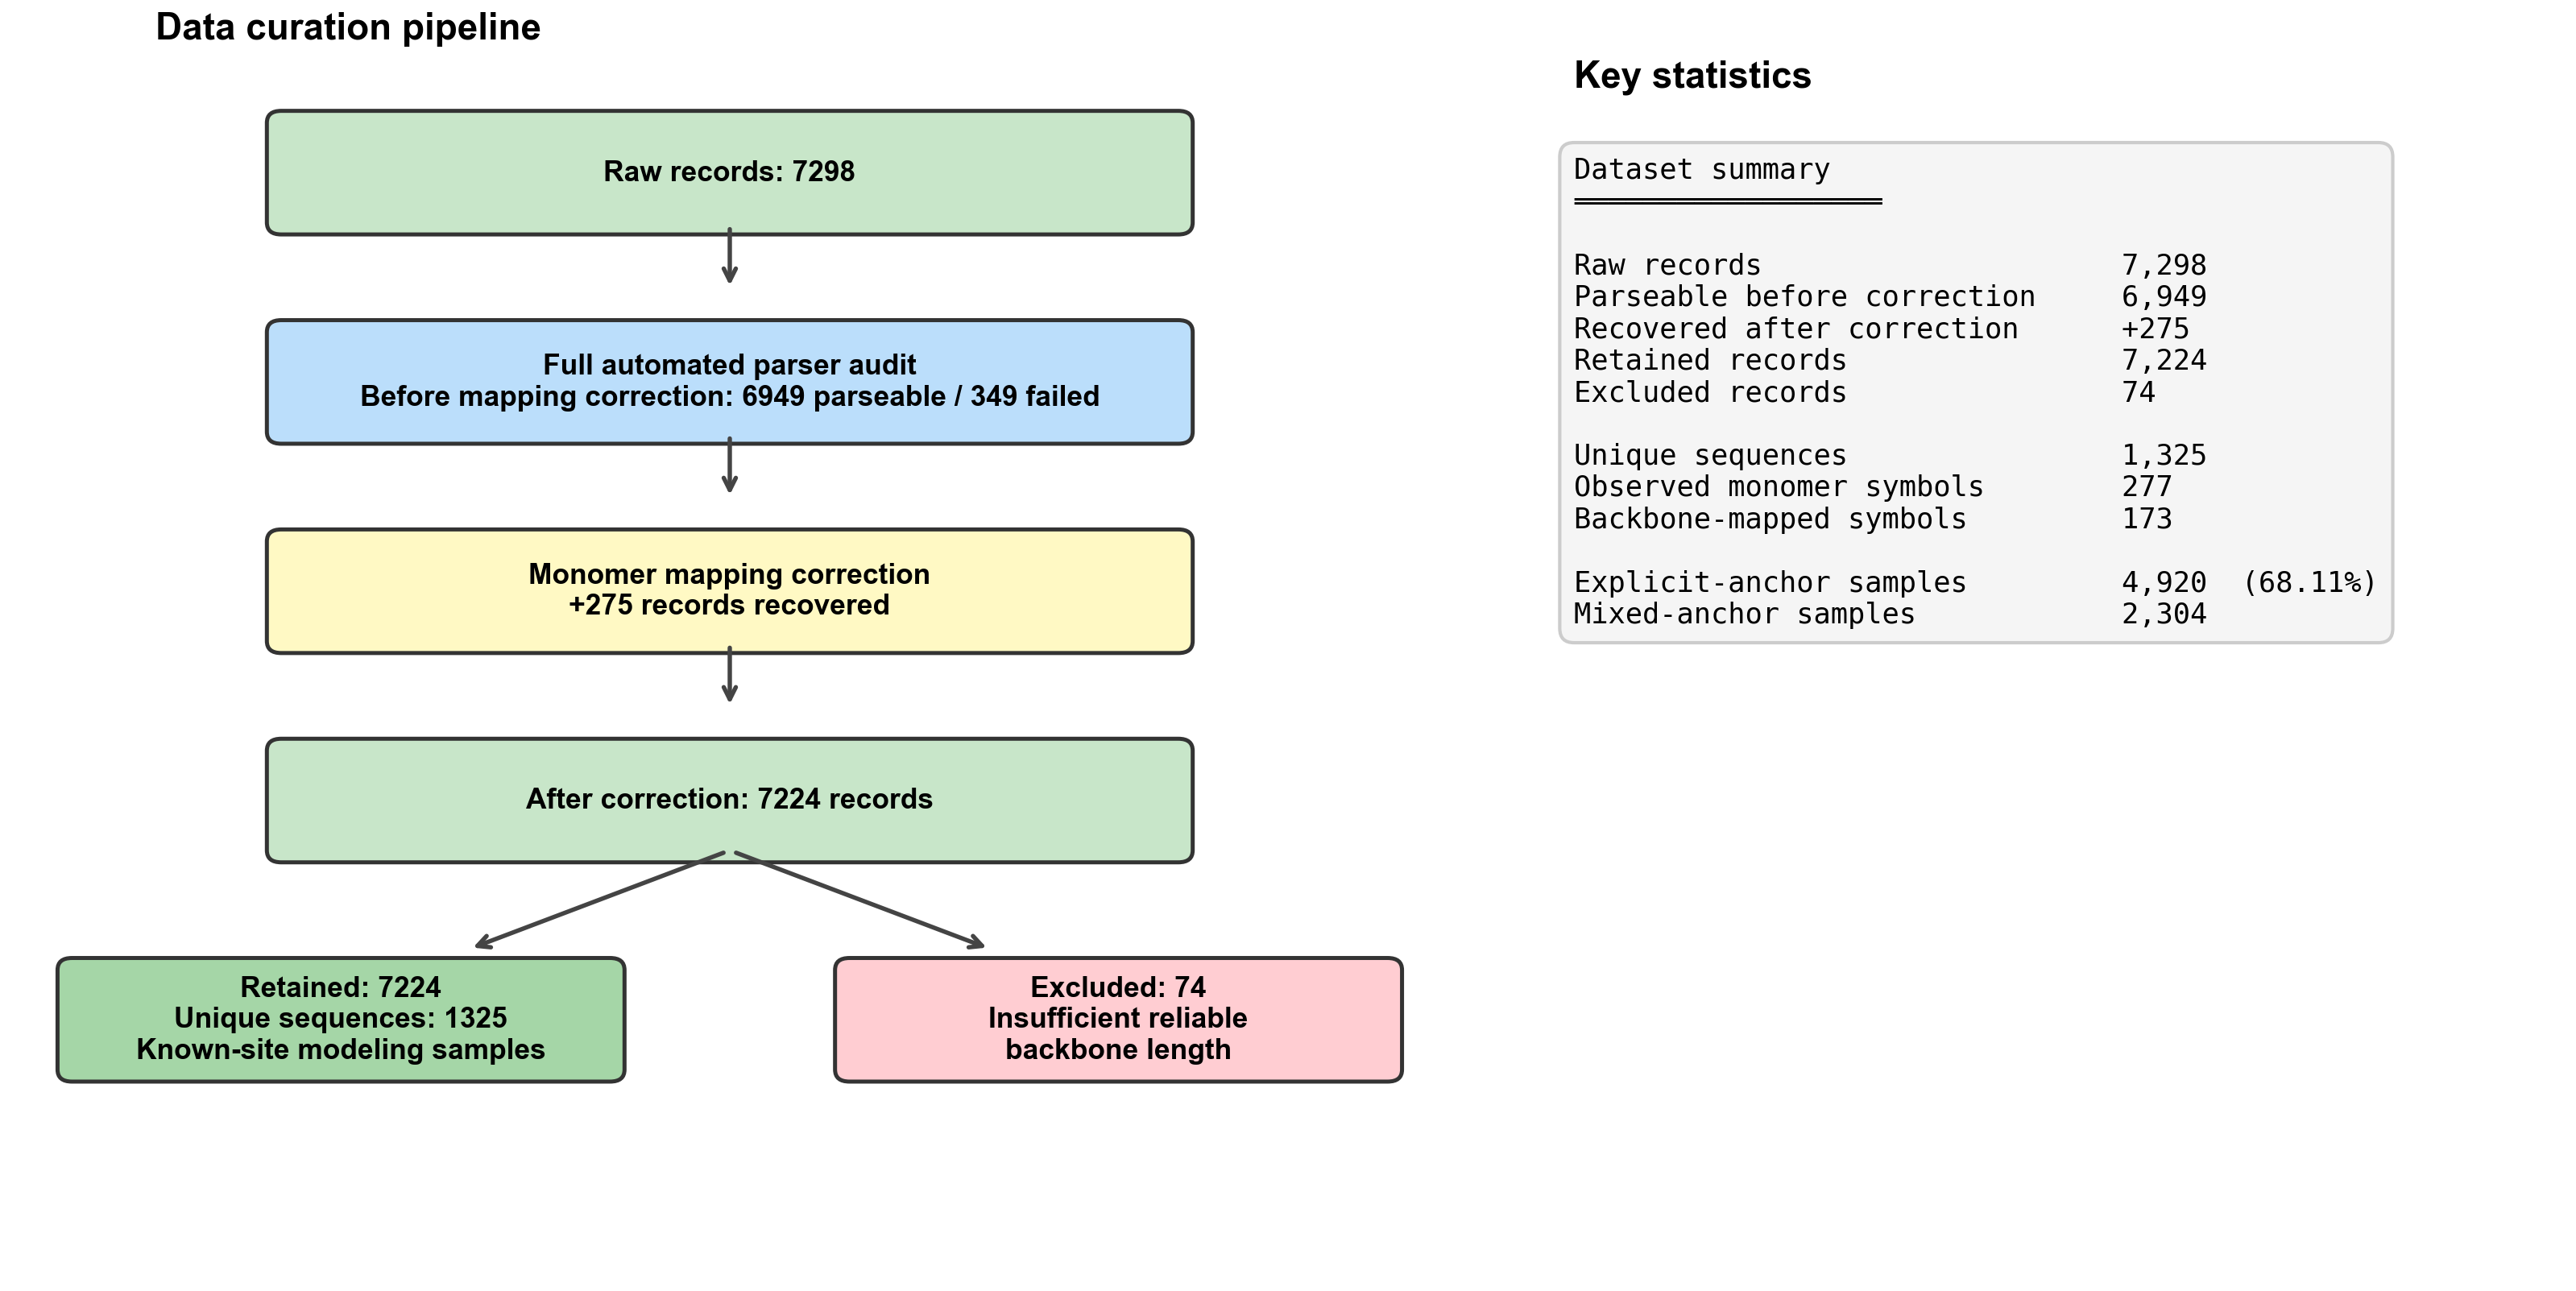
\includegraphics[width=\textwidth]{figures/revision/figS1_parser_audit_flow.pdf}
\caption{%
Parser audit and dataset curation flow.
(\textit{Left}) Data pipeline from raw CycPeptMPDB records through
automated parsing, monomer-mapping correction, and exclusion to the
final known-site modeling dataset.
(\textit{Right}) Key summary statistics.
A total of 7224 records (98.99\%) were retained; 74 records were
excluded because of insufficient reliable backbone length.}
\label{fig:parser_audit_flow}
\end{figure}

% --- Supplementary Figure S2: Site Perturbation Controls ---
\begin{figure}[t]
\centering
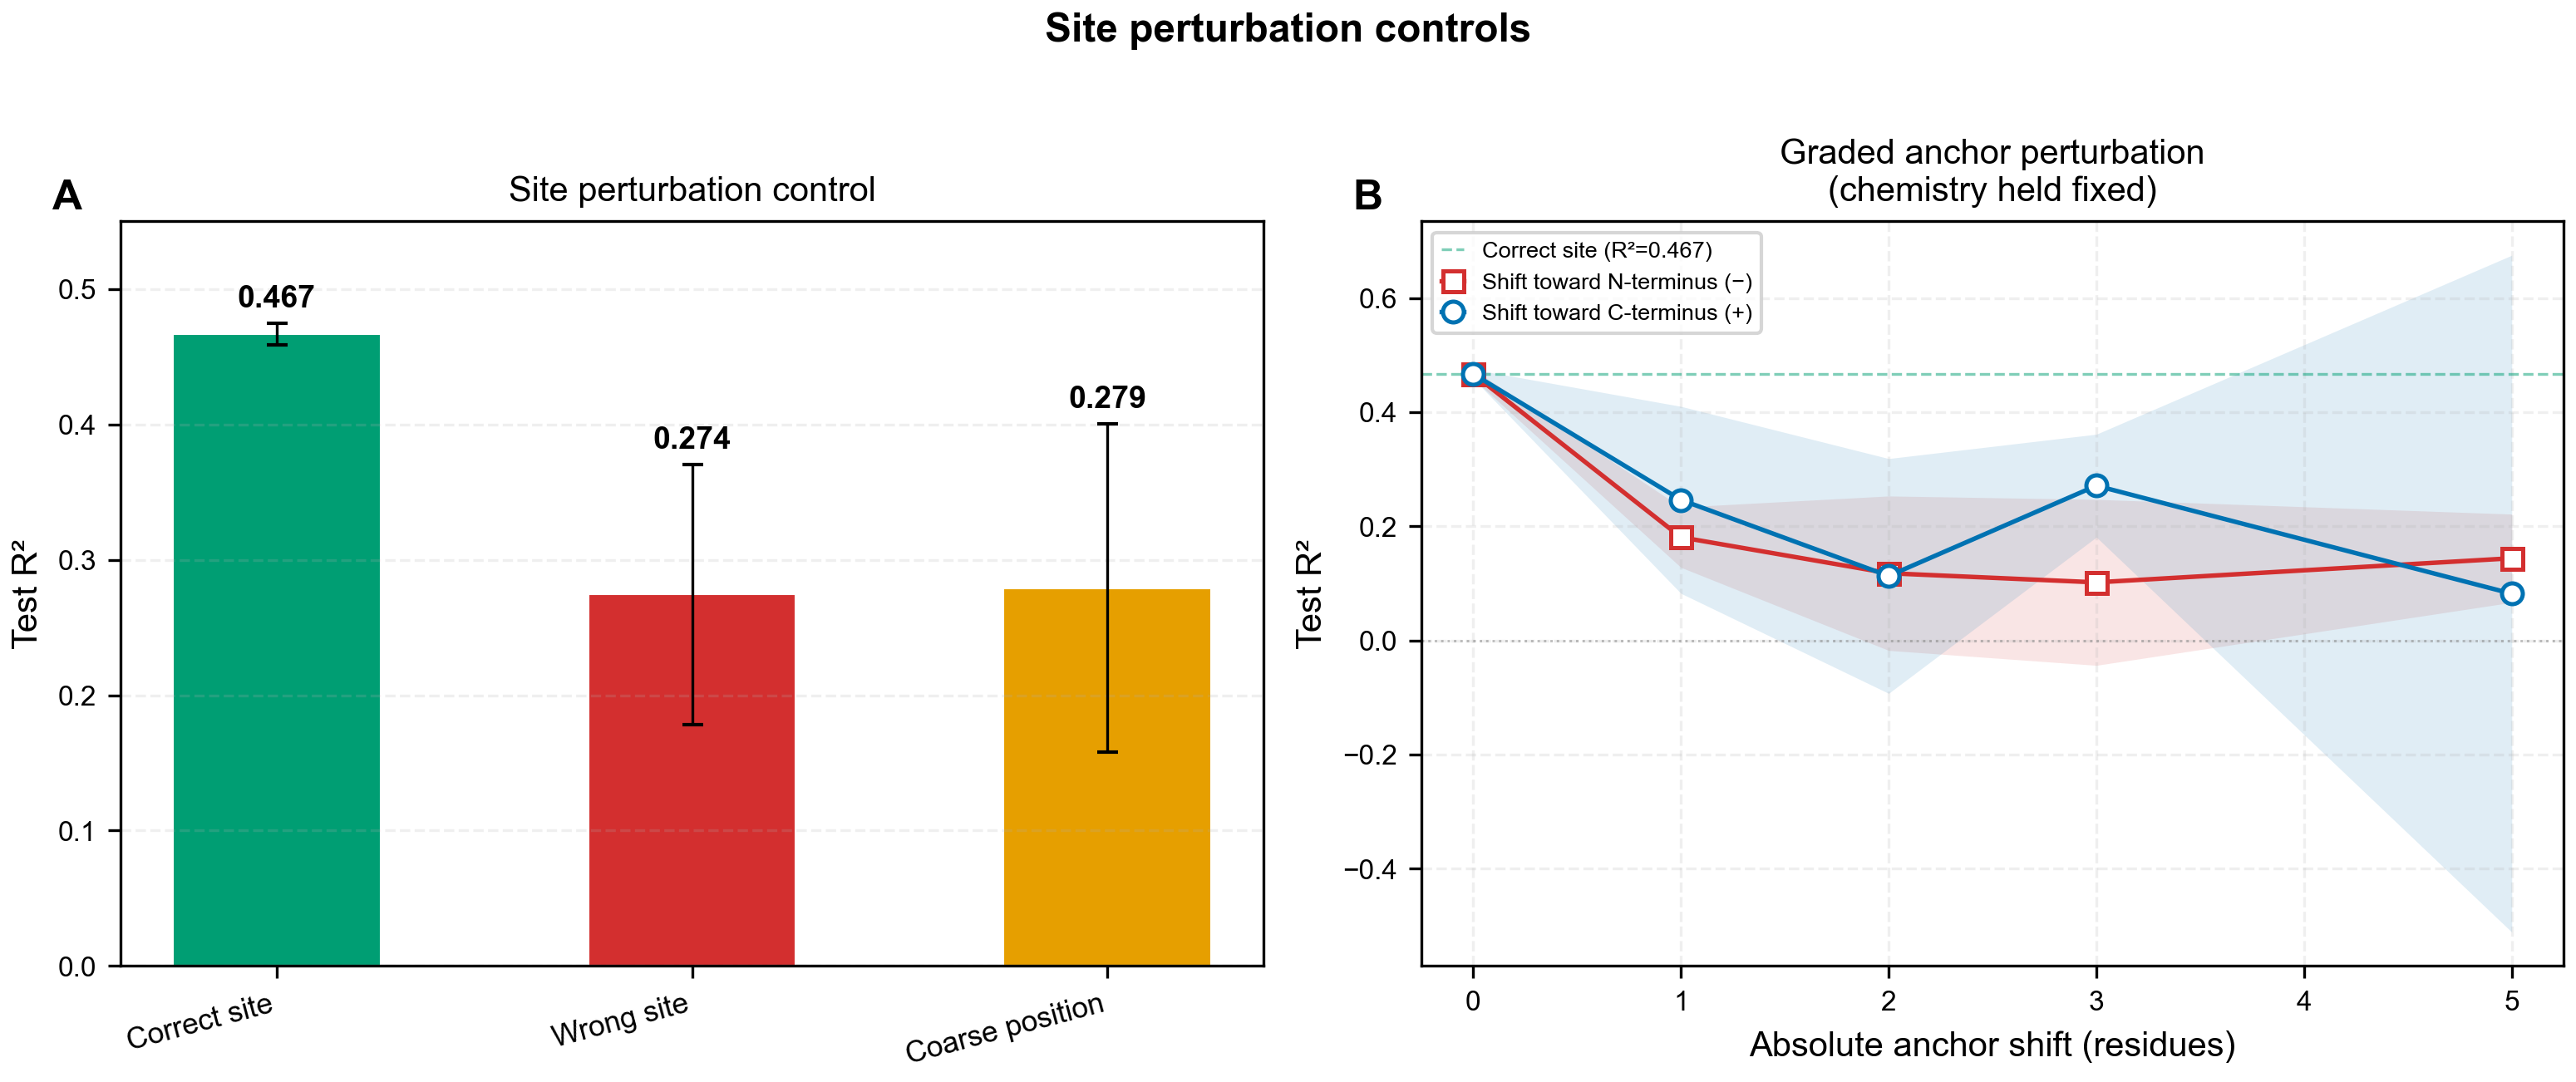
\includegraphics[width=0.92\textwidth]{figures/revision/figS2_site_perturbation_controls.pdf}
\caption{%
Site perturbation controls.
(\textbf{A}) Comparison of correct, wrong (hash-based shift), and
coarse-position (tertile) site encodings.  Both perturbations
significantly degrade test R$^2$.
(\textbf{B}) Graded anchor perturbation: R$^2$ as a function of
absolute residue shift from the correct anchor position.
Edit chemistry was held fixed; only site annotations were perturbed.
Both N-terminal and C-terminal shifts cause rapid performance
collapse, confirming tight coupling between model performance and
accurate site specification.}
\label{fig:site_perturbation_controls}
\end{figure}

% --- Supplementary Figure S3: B-Subblock Ablation ---
\begin{figure}[t]
\centering
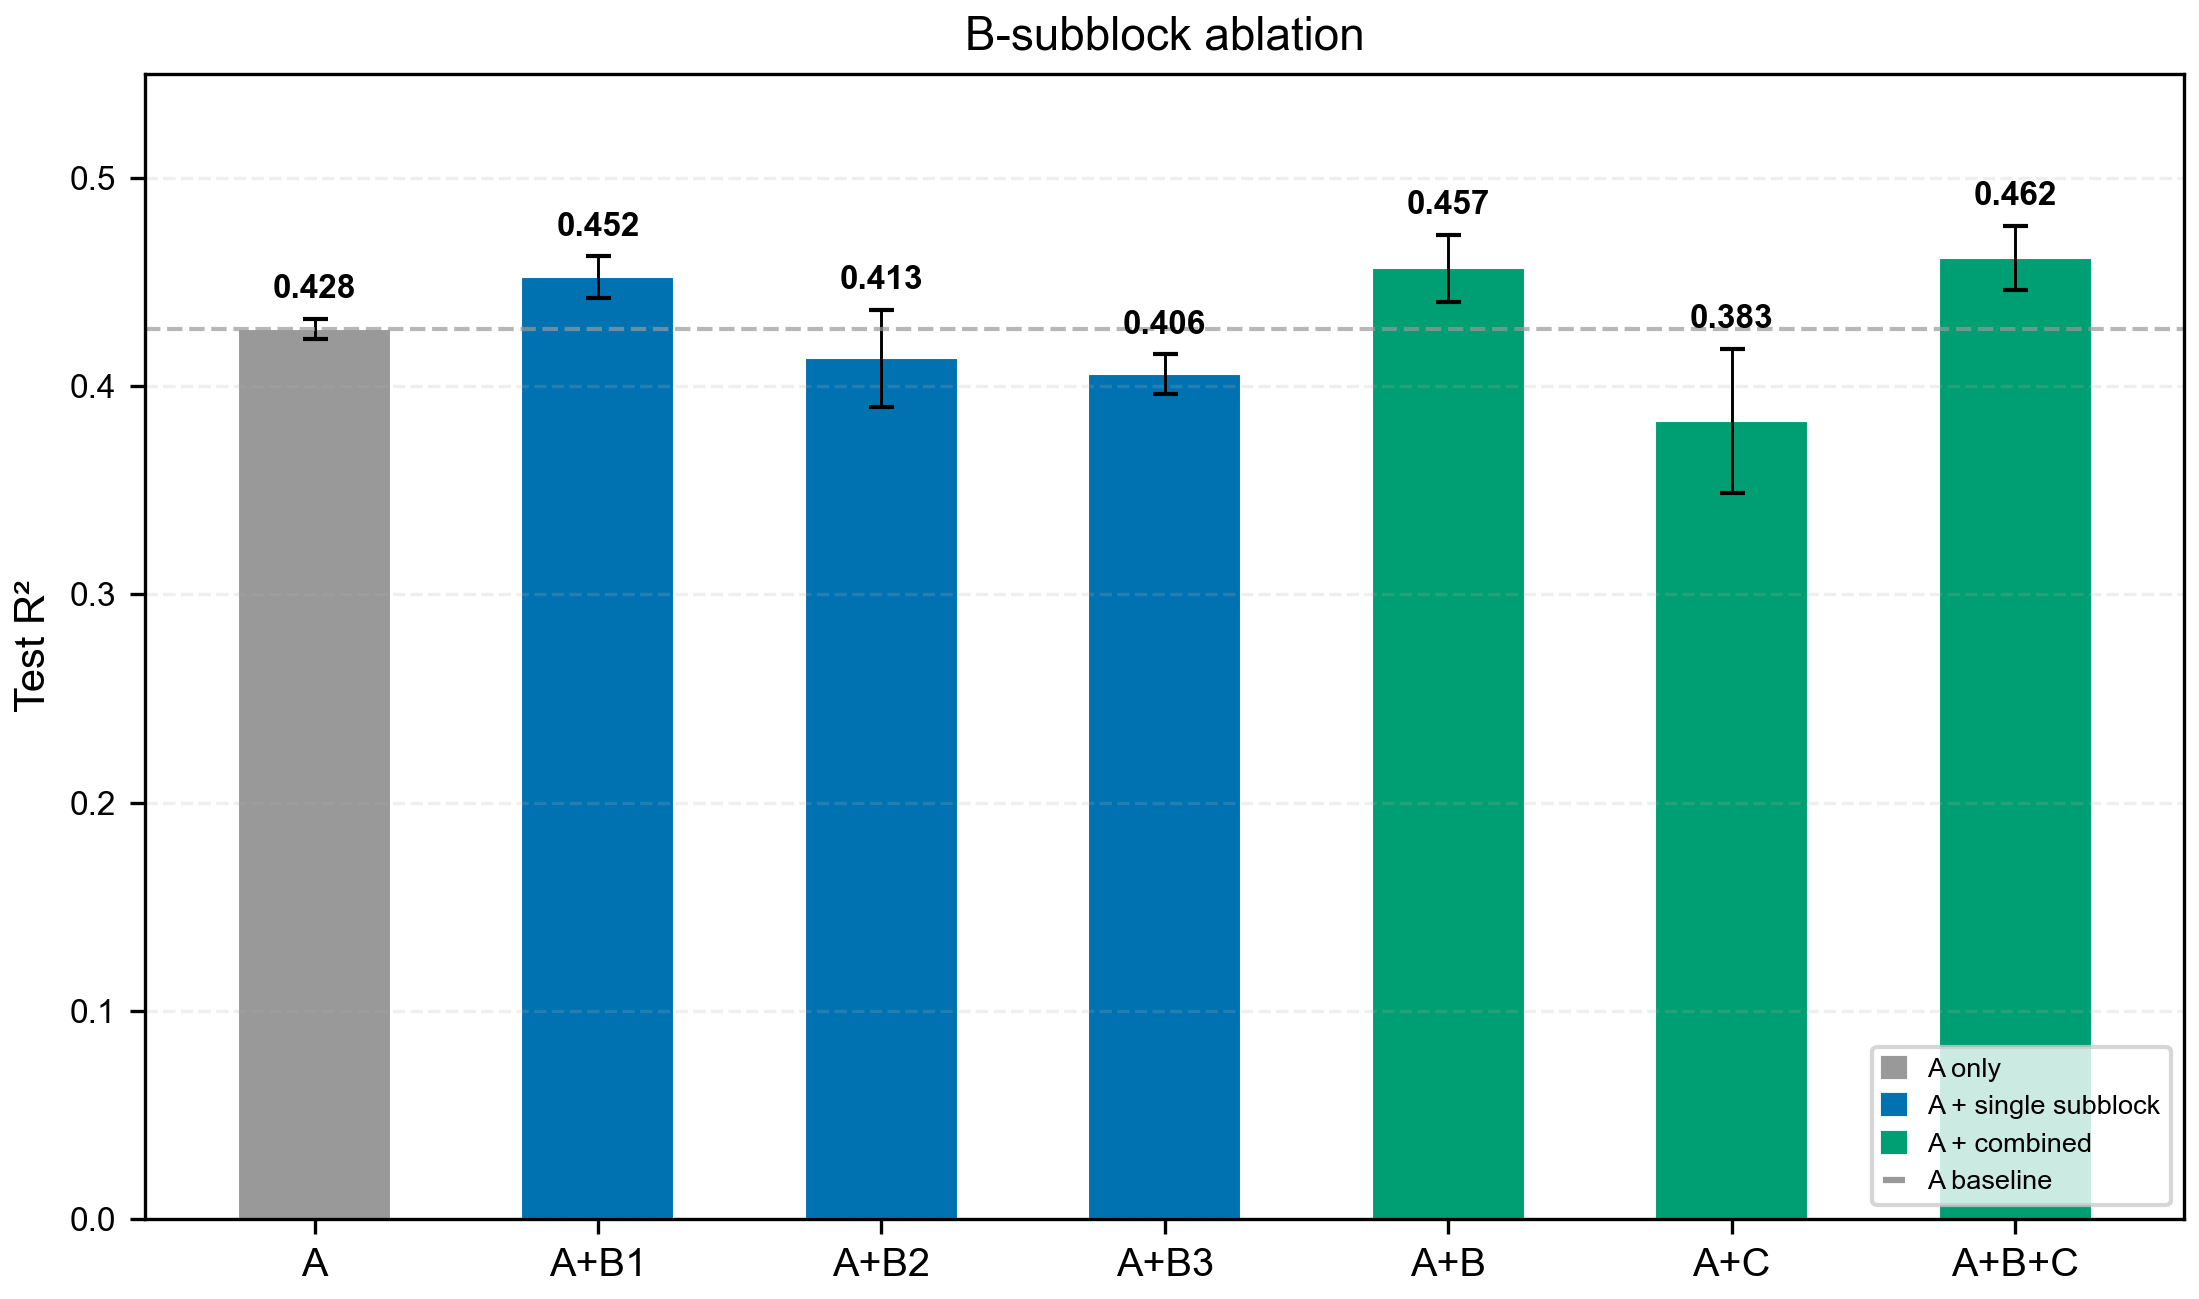
\includegraphics[width=0.88\textwidth]{figures/revision/figS3_B_subblock_ablation.pdf}
\caption{%
B-subblock ablation.  Bars show test R$^2$ for chemistry alone (A),
chemistry plus individual site subblocks (B1: position statistics;
B2: anchor-residue composition; B3: anchor-residue property), and
chemistry with combined site descriptors (A+B), context (A+C), or
all descriptors (A+B+C).  The dashed line marks the A-only baseline.
Position statistics (A+B1) provide the clearest single-subblock
improvement, while the full site descriptor set (A+B) and the
complete model (A+B+C) achieve the largest gains.}
\label{fig:B_subblock_ablation}
\end{figure}

% --- Supplementary Figure S4: Predicted vs Observed ---
%\begin{figure}[t]
%\centering
%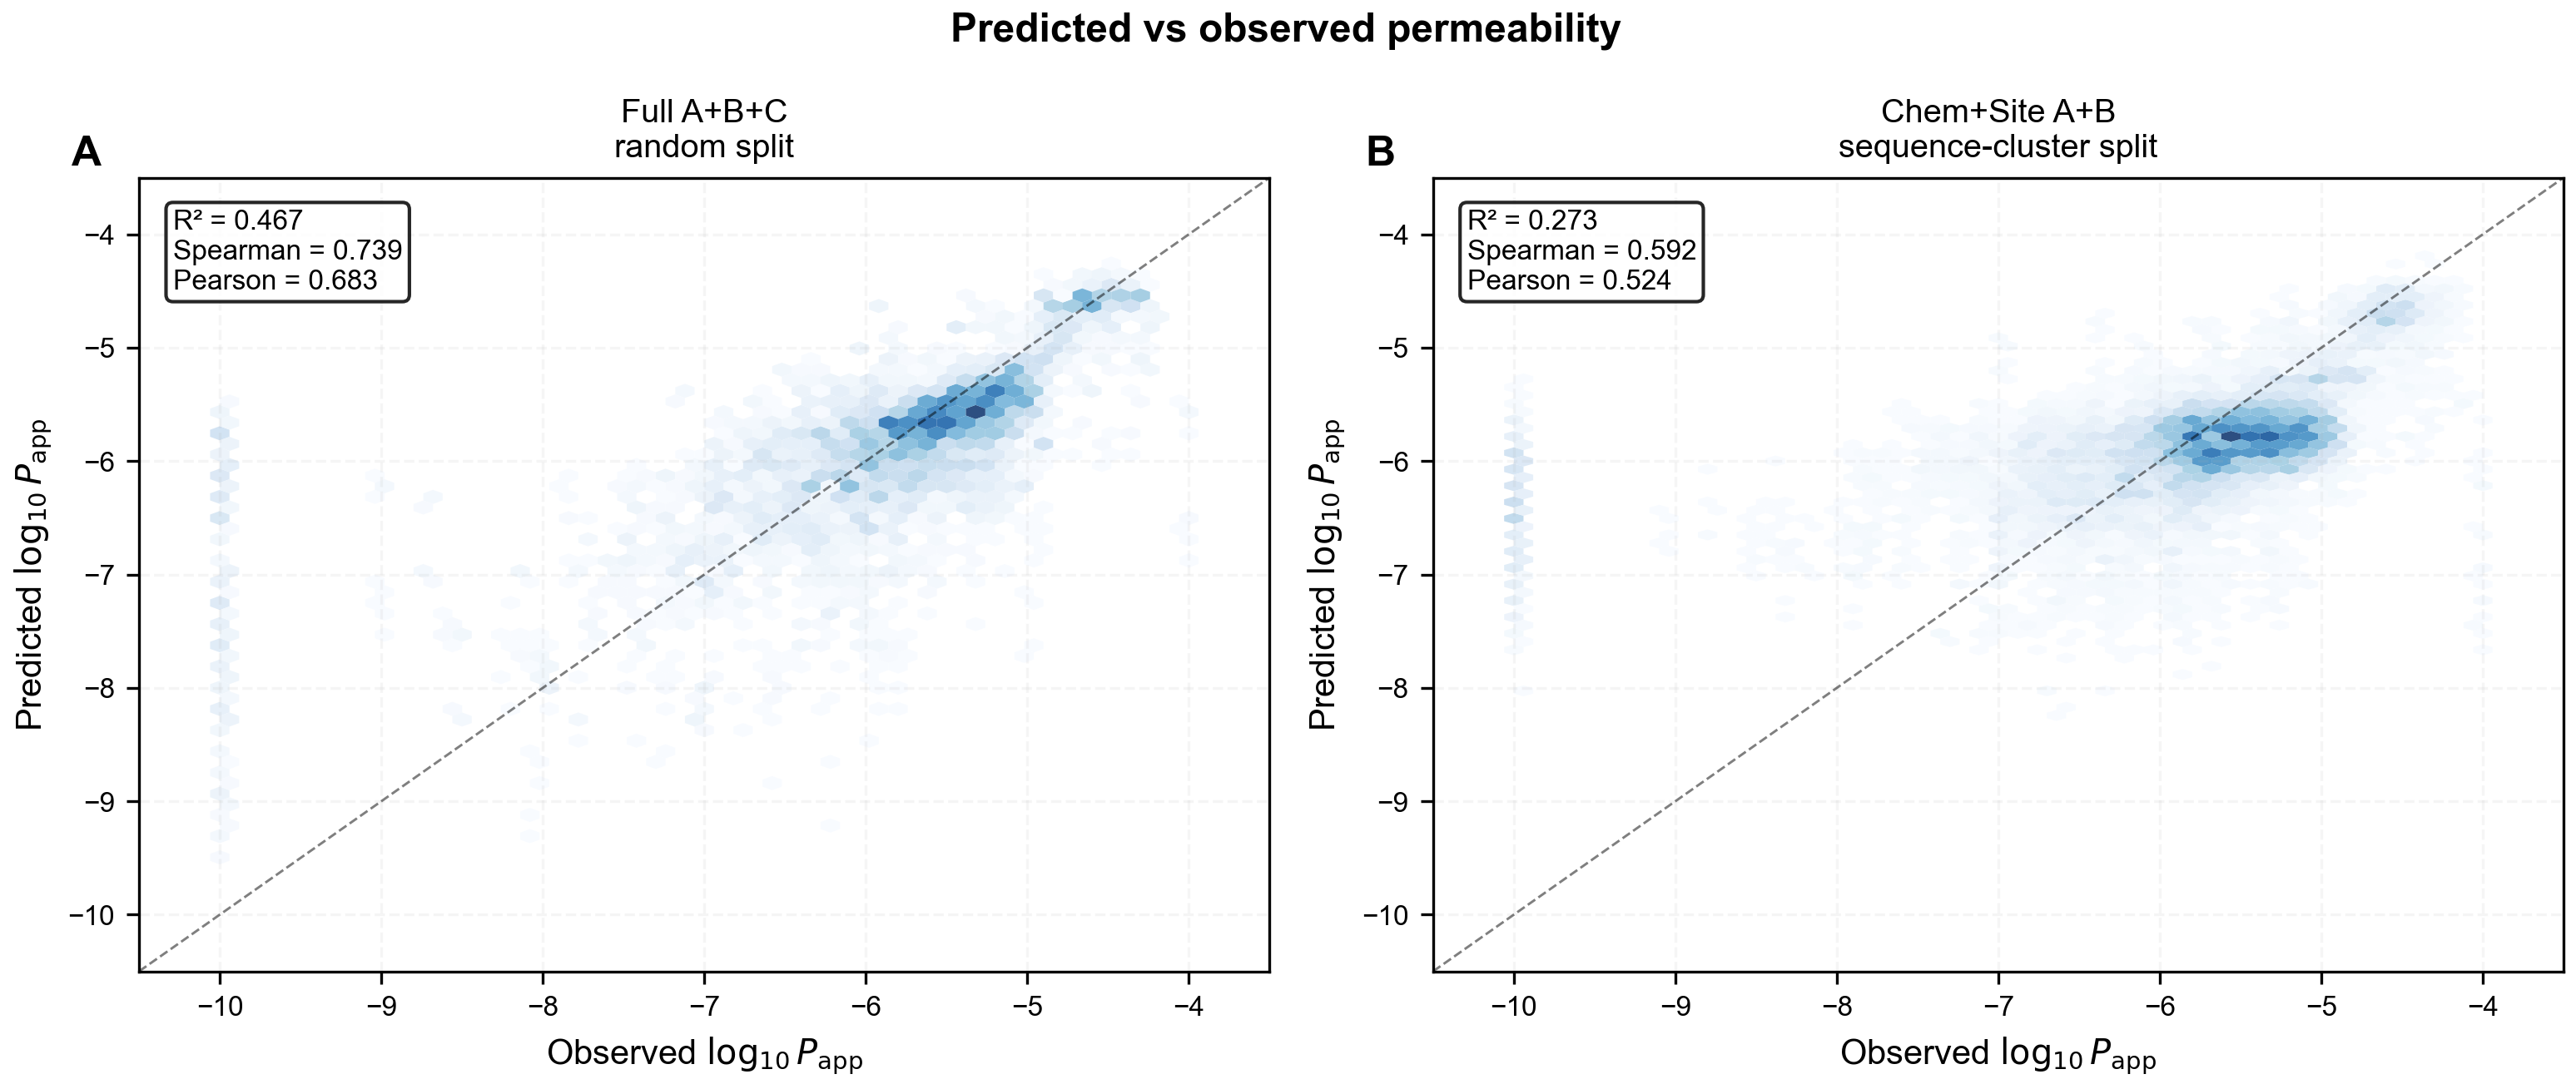
\includegraphics[width=\textwidth]{figures/revision/figS4_predicted_vs_observed.pdf}
%\caption{%
%Predicted versus observed permeability.
%(\textbf{A}) Full A+B+C model on the random split.
%(\textbf{B}) Chem+Site A+B model on the sequence-cluster split.
%The diagonal line marks $y=x$.  R$^2$, Spearman $\rho$, and
%Pearson $r$ are reported in each panel.
%Note: vertical accumulation near $\log_{10}P_{\mathrm{app}}
%\approx -10$ may reflect censored source labels.}
%\label{fig:predicted_vs_observed}
%\end{figure}
